\documentclass{article}

\usepackage{hyperref}
\usepackage{graphicx}
\usepackage{wrapfig}

\newenvironment{code}{\obeycr\begin{it}\nopagebreak\addvspace{1ex}\noindent\footnotesize\begin{tabular}{|p{0.95\textwidth}|}\hline}{\\\hline\end{tabular}\par\addvspace{1ex}\end{it}\restorecr}

\newcommand{\inlinecode}[1]{\textit{#1}}
\newcommand{\Sl}{\textbf{S$_{L}$}}
\newcommand{\Sr}{\textbf{S$_{R}$}}

\title{Red-black trees implementation in Prolog}
\author{Roman Pitak \\ \url{baracudafish@gmail.com}}
\date{2009-06-16}

\begin{document}
\maketitle
\tableofcontents
\newpage
\section[Introduction]{Introduction to red-black trees}
Red-black trees are self-balancing binary search trees. The implementation is complex, but it has a good worst-case running time for its operations and is effective in practice: it can search, insert and delete in O(log n) time, where n is the total number of elements in the tree. In red-black trees the leaf nodes are not relevant and do not contain data. Unlike binary search trees, each node of a red-black tree has a color attribute, the value of which is either red or black. In addition to the ordinary requirements imposed on binary search trees, the following additional requirements of any valid red-black tree apply:

\begin{enumerate}
\item A node is either red or black.
\item The root is black. ( This rule has little effect on the analysis, since the color of the root can always be changed from red to black. )
\item All leaves are black.
\item Both children of every red node are black.
\item Every simple path from a given node to its descendant leaves contains the same number of black nodes.
\end{enumerate}

These constraints enforce a critical property of red-black trees: that the longest path from the root to any leaf is no more than twice as long as the shortest path from the root to any other leaf in that tree. The result is that the tree is roughly balanced. To see why these properties guarantee this, it suffices to note that no path can have two red nodes in a row, due to property 4.

\section{User's manual}
This part of the manual focuses on the usage and functionality of the \inlinecode{rb\_trees.pl} library. 
The algorithms used for the implementation are described later in the Programmers manual\pageref{programmers_manual}.

\subsection{Data structures}
This implementation represents a node in a red-black tree as a tetrad : 
\\\inlinecode{t( Color, Key, LeftSubtree, RightSubtree )} where
\begin{itemize}
  \item[\inlinecode{Color}] represents the color of the node
  \item[\inlinecode{Key}] represents the value stored in the node
  \item[\inlinecode{LeftSubtree}] is the left child of the node
  \item[\inlinecode{RightSubtree}] is the right child of the node, both represented again as a tetrad, or as \inlinecode{nil}, if the node is a leaf.
\end{itemize}
Leaves are represented as a node with the \inlinecode{Key} $=$ \inlinecode{nil} i.e. \inlinecode{t( b, nil, nil, nil )}.

All the data presented to the predicates must obey this format and also satisfy the rules mentioned in the introduction to red-black trees. The \inlinecode{rb\_check} predicate can be used to determine whether your data satisfy all the above mentioned rules.

\subsection{\inlinecode{rb\_check( +Tree ).}}
The \inlinecode{rb\_check} predicate determines whether the given tree is red-black tree valid by the standards of this implementation. The imput is a data structure (presumably a red-black tree) we want to test for the red-black tree properties. It fails if any of the requirements have not been met.

\subsection{\inlinecode{rb\_empty( ?Tree ).}}
The \inlinecode{rb\_empty} predicate, if given a tree succeeds if the tree is empty. If called with an previously ununified `variable', outputs an empty tree: \\\inlinecode{t( b, nil, nil, nil )}.

\subsection{\inlinecode{rb\_insert( +Tree, +Key, -NewTree ).}}
The \inlinecode{rb\_insert} predicate inserts a new node with the given Key into the given Tree and outputs a new tree, preserving all the required red-black tree properties. Note that due to rotions and color changes the new tree may have a different internal structure (this is only visible/important if you print the trees).

\subsection{\inlinecode{rb\_build( +List, -Tree ).}}
The \inlinecode{rb\_build} predicate takes a list of elements and builds a red black tree from scratch.

\subsection{\inlinecode{rb\_delete( +Tree, +Key, -NewTree ).}}
The \inlinecode{rb\_delete} deletes the node with the given Key from the given Tree and outputs a new tree, preserving all the required red-black tree properties. Note that due to rotions and color changes the new tree may have a different internal structure (this is only visible/important if you print the trees).

\subsection{\inlinecode{rb\_search( +Tree, +Element ).}}
The \inlinecode{rb\_search} predicate searches in the given tree for the given element. Fails if the element is not found.

\subsection{\inlinecode{rb\_maximum( +Tree, -Maximum ).}}
The \inlinecode{rb\_maximum} predicate finds the maximal element of the given tree (subtree), or fails if given an empty tree.

\subsection{\inlinecode{rb\_minimum( +Tree, -Minimum ).}}
The \inlinecode{rb\_minimum} predicate finds the minimal element of the given tree (subtree), or fails if given an empty tree.

\subsection{\inlinecode{rb\_inOrder( +Tree, -List ).}}
The \inlinecode{rb\_inOrder} predicate performs an inorder tree traversal of the given tree and outputs a list of it's elements as defined the rules of an inorder tree walk.
Two similar aditional predicates are provided in this implementation:\\
\inlinecode{rb\_preOrder( +Tree, -List ).}\\
\inlinecode{rb\_postOrder( +Tree, -List ).}\\
These perform preorder and postorder tree traversals.

\subsection{\inlinecode{rb\_print( +Tree ).}}
The \inlinecode{rb\_print} predicate prints the given tree on the standars output in a human readable format.
An example of the \inlinecode{rb\_print} output:


{\obeycr\nopagebreak\addvspace{1ex}\noindent\footnotesize\begin{tabular}{|p{0.95\textwidth}|}\hline
[ ] Black node
( ) Red node

\hspace{6ex}\textbar ---(19)
\hspace{1ex}\textbar ---[16]
\hspace{1ex}\textbar \hspace{4ex}\textbar ---(15)
[12]
\hspace{1ex}\textbar \hspace{9ex}\textbar ---(11)
\hspace{1ex}\textbar \hspace{4ex}\textbar ---[10]
\hspace{1ex}\textbar \hspace{4ex}\textbar \hspace{4ex}\textbar ---(9)
\hspace{1ex}\textbar ---(5)
\hspace{6ex}\textbar \hspace{4ex}\textbar ---(3)
\hspace{6ex}\textbar ---[2]
\hspace{11ex}\textbar ---(1)
\\\hline\end{tabular}\par\addvspace{1ex}\restorecr}

\pagebreak
\section{Programmer's manual}
\label{programmers_manual}
Read-only operations on a red-black tree require no modification from those used for binary search trees, because every red-black tree is a special case of a simple binary search tree. However, the immediate result of an insertion or removal may violate the properties of a red-black tree. Therefore a small number of color changes and no more than three tree rotations may be required.

\subsection{Read-only operations}
\subsubsection{Search}
The \inlinecode{rb\_search} predicate searches the given \inlinecode{Tree} for the given \inlinecode{Element} in \\O(log n) time using the binary search tree properties of a red-black tree.

\begin{code}
\% rb\_search( +Tree, +Element ).\\
rb\_search( t( b, nil, nil, nil ), \_ ) :- !, fail.\\
rb\_search( t( \_, K, \_, \_ ), K ).\\
rb\_search( t( \_, K, Ls, \_ ), Ks ) :-
\hspace{2ex}K $>$ Ks,
\hspace{2ex}rb\_search( Ls, Ks ).\\
rb\_search( t( \_, K, \_, Rs ), Ks ) :-
\hspace{2ex}K $<$ Ks,
\hspace{2ex}rb\_search( Rs, Ks ).
\end{code}

\subsubsection{Minimum}
The \inlinecode{rb\_minimum} predicate finds the minimal element of the given \inlinecode{Tree} (\inlinecode{subree}). That can be achieved by going `left' in the tree structure.

\begin{code}
\% rb\_minimum( +Tree, -Minimum ).
\% fails on empty !
rb\_minimum( t( \_, K, t( b, nil, nil, nil ), \_ ), K ).
rb\_minimum( t( \_, \_, Ls, \_ ), Minimum ) :-
\hspace{2ex}rb\_minimum( Ls, Minimum ).
\end{code}

\subsubsection{Maximum}
The \inlinecode{rb\_maximum} predicate finds the maximal element of the given \inlinecode{Tree} (\inlinecode{subtree}). That can be achieved by going `right' in the tree structure.

\begin{code}
\% rb\_maximum( +Tree, -Maximum ).
\% fails on empty !
rb\_maximum( t( \_, K, \_, t( b, nil, nil, nil ) ), K ).
rb\_maximum( t( \_, \_, \_, Rs ), Maximum ) :-
\hspace{2ex}rb\_maximum( Rs, Maximum ).
\end{code}

\subsubsection[Inorder]{Inorder tree traversal}
The \inlinecode{rb\_inOrder} predicate performs an inorder tree traversal of the given \inlinecode{Tree} by appending the Key of the actual node after the result of the inorder traversal of the left subtree and before the result of the inorder traversal of the right subtree. Resulting in a sorted list of the \inlinecode{Tree} elements.

\begin{code}
\% rb\_inOrder( +Tree, -List ).\\
rb\_inOrder( t( b, nil, nil, nil ), [] ).\\
rb\_inOrder( t( \_, K, Ls, Rs ), L ) :-
\hspace{2ex}rb\_inOrder( Ls, Ll ), 
\hspace{2ex}rb\_inOrder( Rs, Lr ),
\hspace{2ex}append( Ll, [ K \textbar Lr ], L ).
\end{code}

\subsubsection[Preorder]{Preorder tree traversal}
The \inlinecode{rb\_preOrder} predicate performs a preorder tree traversal of the given \inlinecode{Tree}.

\begin{code}
\% rb\_preOrder( +Tree, -List ).\\
rb\_preOrder( t( b, nil, nil, nil ), [] ).\\
rb\_preOrder( t( \_, K, Ls, Rs ), L ) :-
\hspace{2ex}rb\_preOrder( Ls, Ll ), 
\hspace{2ex}rb\_preOrder( Rs, Lr ),
\hspace{2ex}append( [ K \textbar Ll ], Lr, L ).
\end{code}

\subsubsection[Postorder]{Postorder tree traversal}
The \inlinecode{rb\_postOrder} predicate performs a postorder tree traversal of the given \inlinecode{Tree}.

\begin{code}
\% rb\_postOrder( +Tree, -List ).\\
rb\_postOrder( t( b, nil, nil, nil ), [] ).\\
rb\_postOrder( t( \_, K, Ls, Rs ), L ) :-\\
\hspace{2ex}rb\_postOrder( Ls, Ll ), 
\hspace{2ex}rb\_postOrder( Rs, Lr ),
\hspace{2ex}append( Ll, Lr, Lp ), 
\hspace{2ex}append( Lp, [ K ], L ).
\end{code}

\subsubsection{Print}
The \inlinecode{rb\_print} predicate offers a way to print a red-black tree in a `human readable' format. It performs a reversed inorder tree traversal printing `on the go'.
Each color of a tree node has it's unique representation:
\begin{itemize}
\item[(1)]It prints the Key of a red node in parentheses, 
\item[{[2]}]the Key of a black node in square brackets 
\item[\{3\}]and the Key of a double black node in curly brackets.
\end{itemize}
\nopagebreak
Note: what a doble black node is will be explained later in the Delete section\ref{double_black}.

\begin{code}
\% rb\_print( +Tree ).\\
rb\_print( T ) :-
\hspace{2ex}write( '[ ] Black node' ), nl, 
\hspace{2ex}write( '( ) Red node' ), nl, nl,
\hspace{2ex}rb\_print( T, [] , nodebug ), nl, !.\\
\end{code}

\inlinecode{rb\_print} offers two modes of printing:
\begin{itemize}
\item{debug} mode may be used while debuging parts of the program, while it also prints the `empty' black leaves. The result is a rather `longer' tree, but possible leaf errors may be seen.
\item{no debug} mode prints a nice compact tree.
\end{itemize}
The printing mode can only be secified in the code above.

\begin{code}
rb\_print( t( b, nil, nil, nil ), \_, nodebug ).\\
rb\_print( nil, N , debug ) :- !, 
\hspace{2ex}rb\_spaces( N ), write( 'nil' ), nl.\\
rb\_print( t( b, nil, Ls, Rs ), N , debug ) :- 
\hspace{2ex}append( N, [ 'r' ], Nr ), rb\_print( Rs, Nr , debug ), !, 
\hspace{2ex}rb\_spaces( N ), put( '[' ), write( nil ), put( ']' ), nl,
\hspace{2ex}append( N, [ 'l' ], Nl ), rb\_print( Ls, Nl , debug ), !.\\
rb\_print( t( b, K, Ls, Rs ), N , D ) :-
\hspace{2ex}append( N, [ 'r' ], Nr ), rb\_print( Rs, Nr , D ), !, 
\hspace{2ex}rb\_spaces( N ), put( '[' ), write( K ), put( ']' ), nl,
\hspace{2ex}append( N, [ 'l' ], Nl ), rb\_print( Ls, Nl , D ), !.\\
rb\_print( t( r, K, Ls, Rs ), N , D ) :-
\hspace{2ex}append( N, [ 'r' ], Nr ), rb\_print( Rs, Nr , D ), !, 
\hspace{2ex}rb\_spaces( N ), put( '(' ), write( K ), put( ')' ), nl,
\hspace{2ex}append( N, [ 'l' ], Nl ), rb\_print( Ls, Nl , D ), !.\\
rb\_print( t( bb, K, Ls, Rs ), N , D ) :-
\hspace{2ex}append( N, [ 'r' ], Nr ), rb\_print( Rs, Nr , D ), !, 
\hspace{2ex}rb\_spaces( N ), put( '{' ), write( K ), put( '}' ), nl,
\hspace{2ex}append( N, [ 'l' ], Nl ), rb\_print( Ls, Nl , D ), !.
\end{code}

The \inlinecode{rb\_spaces} predicate prints the indentation of the nodes, while adding edges to the picture resulting in a more readable representation. A `\textbar' is added only on `direction changes' and a `\hspace{1ex}\textbar---' is printed right before the node (at the end of the indentation).

\begin{code}
rb\_spaces( [] ).\\
rb\_spaces( [ \_ ] ) :- 
\hspace{2ex}write( '\hspace{1ex}\textbar---' ).\\
rb\_spaces( [ H, H \textbar T ] ) :-
\hspace{2ex}write( '\hspace{5ex}' ), 
\hspace{2ex}rb\_spaces( [ H \textbar T ] ).\\
rb\_spaces( [ \_ \textbar T ] ) :-
\hspace{2ex}write( '\hspace{1ex}\textbar\hspace{3ex}' ), 
\hspace{2ex}rb\_spaces( T ).
\end{code}

\subsubsection[Validity]{Red-black tree properties validity check}
The \inlinecode{rb\_check} predicate takes the Tree, checks if the root is black and sends it to the \inlinecode{rb\_ch} predicate. The \inlinecode{rb\_ch} predicate then checks if all the requirements of a red-black tree have been met.

\begin{code}
\% rb\_check( +Tree ).
rb\_check( t( b, K, Ls, Rs ) ) :-
\hspace{2ex}rb\_ch( t( b, K, Ls, Rs ), true, \_ ),
\hspace{2ex}write( 'rb\_check successfull' ), nl.
\end{code}

\begin{itemize}
\item A black empty tree is valid and has one black node in it's path. 
\item On a node with no children the only requirement is that the Key doesn't unify with `nil'. Also there are two black nodes in the path : the node itself and it's black leaf.
\end{itemize}

\begin{code}
\% rb\_ch( +Tree, -Validity, -NumberOfBlackNodes ).
\% Nbn - number of black nodes

rb\_ch( t( b, nil, nil, nil ), true, 1 ).

\% black node with no children (subtrees).
rb\_ch( t( b, K, t( b, nil, nil, nil ), t( b, nil, nil, nil ) ), true, 2 ) :- !, 
\hspace{2ex}K \textbackslash{}= nil.
\end{code}

\begin{itemize}
\item
A black node with a left child (subtree) is valid if it's child is valid, the color of the child is red and the Key of the child is smaller than the Key of the node.
\end{itemize}

\begin{code}
\% black node with a left child
rb\_ch( t( b, K, t( r, Kl, Lsl, Rsl ), t( b, nil, nil, nil ) ), true, 2 ) :- !, 
\hspace{2ex}rb\_ch( t( r, Kl, Lsl, Rsl ), Bl, Nl ), !, 
\hspace{2ex}Bl = true,
\hspace{2ex}Nl = 1,
\hspace{2ex}K \textbackslash{}= nil,
\hspace{2ex}Kl \textbackslash{}= nil,
\hspace{2ex}K \textgreater{} Kl.
\end{code}

\begin{itemize}
\item
For a black node with a right child the only difference from a black node with a left child is that the Key of the child must be greater than that of the parrent.
\end{itemize}

\begin{code}
\% black node with a right child
rb\_ch( t( b, K, t( b, nil, nil, nil ), t( r, Kr, Lsr, Rsr ) ), true, 2 ) :- !, 
\hspace{2ex}rb\_ch( t( r, Kr, Lsr, Rsr ), Br, Nr ), !, 
\hspace{2ex}Br = true,
\hspace{2ex}Nr = 1,
\hspace{2ex}K \textbackslash{}= nil,
\hspace{2ex}Kr \textbackslash{}= nil,
\hspace{2ex}K \textless{} Kr.
\end{code}

\begin{itemize}
\item
For a black node with both children, the children must be valid for themselves and the count of black nodes in each path of the left child must equal the count of the black nodes in each path of the right child. Also the Key values must meet the requirement for a binary search tree.
\end{itemize}

\begin{code}
\% black node with both children
rb\_ch( t( b, K, t( Cl, Kl, Lsl, Rsl ), t( Cr, Kr, Lsr, Rsr ) ), true, N ) :- !, 
\hspace{2ex}rb\_ch( t( Cl, Kl, Lsl, Rsl ), Bl, Nl ), !, 
\hspace{2ex}rb\_ch( t( Cr, Kr, Lsr, Rsr ), Br, Nr ), !, 
\hspace{2ex}Bl = true, 
\hspace{2ex}Br = true,
\hspace{2ex}Nl = Nr,
\hspace{2ex}N is Nl + 1,
\hspace{2ex}K \textbackslash{}= nil,
\hspace{2ex}Kl \textbackslash{}= nil,
\hspace{2ex}Kr \textbackslash{}= nil,
\hspace{2ex}K \textgreater{} Kl, 
\hspace{2ex}K \textless{} Kr.  
\end{code}

\begin{itemize}
\item
A red node with no children is valid if the Key is not `nil'. It has one black node in each path.
\end{itemize}

\begin{code}
\% red node with no children
rb\_ch( t( r, K, t( b, nil, nil, nil ), t( b, nil, nil, nil ) ), true, 1 ) :- !, 
\hspace{2ex}K \textbackslash{}= nil.
\end{code}

\begin{itemize}
\item
A red node with an `only-child' is never to be found in a red-black tree, because it always violates Property 5 (Every simple path from a given node to its descendant leaves contains the same number of black nodes). 
\item
The last valid possibility is a red node with both children. They both have to be black and valid and the count of black nodes in each path of the left child must equal the count of the black nodes in each path of the right child.
\end{itemize}

\begin{code}
\% red node with both children
rb\_ch( t( r, K, t( b, Kl, Lsl, Rsl ), t( b, Kr, Lsr, Rsr ) ), true, N ) :- !, 
\hspace{2ex}rb\_ch( t( b, Kl, Lsl, Rsl ), Bl, Nl ), !, 
\hspace{2ex}rb\_ch( t( b, Kr, Lsr, Rsr ), Br, Nr ), !, 
\hspace{2ex}Bl = true, 
\hspace{2ex}Br = true,
\hspace{2ex}Nl = Nr,
\hspace{2ex}N is Nl + 0,
\hspace{2ex}K \textbackslash{}= nil,
\hspace{2ex}Kl \textbackslash{}= nil,
\hspace{2ex}Kr \textbackslash{}= nil,
\hspace{2ex}K \textgreater{} Kl, 
\hspace{2ex}K \textless{} Kr.
\end{code}

\begin{itemize}
\item
The \inlinecode{default false} case only unifies if none of the  previous (valid) predicates did, which denotes the given subtree \textbf{T} `invalid'. \textbf{T} is printed for debuging purposes and and the predicate \inlinecode{rb\_check} fails.
\end{itemize}

\begin{code}
\% default FALSE
rb\_ch( T, false, 0 ) :- !, 
\hspace{2ex}rb\_print( T ).
\end{code}

\pagebreak
\subsection{Insertion}
The insertion begins by adding a node much as we would in a simple binary search tree and coloring it red, but instead of adding a leaf we add a red interior node with two black leaves in place of an existing black leaf. 

\subsubsection[\inlinecode{rb-insert}]{\inlinecode{rb-insert}}
\begin{code}
\% rb-insert( +Tree, +Key, -Tree ).\\
rb-insert( T1, K, T3 ) :-
\hspace{2ex} rb-ins( T1, K, T2 ), 
\hspace{2ex} rb-reblackRoot( T2, T3 ), !.\\
\% rb-ins( +Tree, +Key, -Tree ).\\
rb-ins( t( b, nil, nil, nil ), K, t( r, K, t( b, nil, nil, nil ), t( b, nil, nil, nil ) ) ).\\
rb-ins( t( C, K, Ls, Rs ), K, t( C, K, Ls, Rs ) ).\\
rb-ins( t( C, K, Ls, Rs ), Ki, Tfixed ) :-
\hspace{2ex} K $<$ Ki,
\hspace{2ex} rb-ins( Rs, Ki, Rsi ),
\hspace{2ex} rb-insFixup( t( C, K, Ls, Rsi ), Tfixed ).\\
rb-ins( t( C, K, Ls, Rs ), Ki, Tfixed ) :-
\hspace{2ex} K $>$ Ki,
\hspace{2ex} rb-ins( Ls, Ki, Lsi ),
\hspace{2ex} rb-insFixup( t( C, K, Lsi, Rs ), Tfixed ).\\
\% rb-reblackRoot( +Tree, -Tree ).
rb-reblackRoot( t( \_, K, Ls, Rs ), t( b, K, Ls, Rs ) ).
\end{code}

After each insertion an insert fixup procedure is called to perform rotations and color changes. What happens next depends on the color of the nearby nodes. The term `uncle node' will be used to refer to the sibling of a nodes parrent, as in human family trees. Note that:
\begin{itemize}
\item[Property 3](All leaves are black) always holds.
\item[Property 4](Both children of every red node are black) is threatened only by adding a red node, repainting a black node red, or a rotation.
\item[Property 5](All paths from any given node to its leaf nodes contain the same number of black nodes) is threatened only by adding a black node, repainting a red node black, or a rotation.
\item The label \textbf{N} will be used to denote the node being inserted, \textbf{P} will denote \textbf{N}'s parent node, \textbf{G} will denote \textbf{N}'s grandparent, and \textbf{U} will denote \textbf{N}'s uncle.
\end{itemize}

\subsubsection[\inlinecode{rb-insFixup}]{Insert fixup}
Several cases may occur, depending on the position of the inserted node:
\paragraph{Case 1}
The new node \textbf{N} is at the root of the tree. In this case, \textbf{N} is repainted black to satisfy Property 2 (The root is black). Since this adds one black node to every path at once, Property 5 (All paths from any given node to its leaf nodes contain the same number of black nodes) is not violated.
\paragraph{Case 2}
The new node's parent \textbf{P} is black, so Property 4 (Both children of every red node are black) is not invalidated. In this case, the tree is still valid. Property 5 (All paths from any given node to its leaf nodes contain the same number of black nodes) is not threatened, because \textbf{N} is red.

\begin{figure}[h]
\begin{wrapfigure}{r}{0.5\textwidth}
  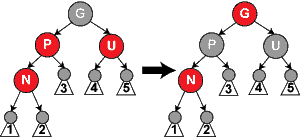
\includegraphics[width=0.5\textwidth]{Red-black_tree_insert_case_3}
  \caption{Transformation of a red-black subtree in case 3 of the insert fixup.}
  \label{insFix3}
\end{wrapfigure}
\paragraph{Case 3}
If both the parent \textbf{P} and the uncle \textbf{U} are red, then both nodes can be repainted black and the grandparent \textbf{G} becomes red (to maintain Property 5 (All paths from any given node to its leaf nodes contain the same number of black nodes)). Now, the new red node \textbf{N} has a black parent. Since any path through the parent or uncle must pass through the grandparent, the number of black nodes on these paths has not changed. However, the grandparent \textbf{G} may now violate properties 2 (The root is black) or 4 (Both children of every red node are black). To fix this, this procedure is recursively performed on \textbf{G}.
Four symmetrical cases had to be implemented in the code (\textbf{P} being \textbf{G}'s left or right child and \textbf{N} being \textbf{P}'s left or right child.)
\end{figure}

\begin{code}
\% CASE \#3\\
rb-insFixup( t( b, Kz, t( r, Ky, t( r, Kx, Lsx, Rsx ), Rsy ), t( r, Ku, Lsu, Rsu ) ), t( r, Kz, t( b, Ky, t( r, Kx, Lsx, Rsx ), Rsy ), t( b, Ku, Lsu, Rsu ) ) ).\\
rb-insFixup( t( b, Kz, t( r, Ky, Lsy, t( r, Kx, Lsx, Rsx ) ), t( r, Ku, Lsu, Rsu ) ), t( r, Kz, t( b, Ky, Lsy, t( r, Kx, Lsx, Rsx ) ), t( b, Ku, Lsu, Rsu ) ) ).\\
rb-insFixup( t( b, Kz, t( r, Ku, Lsu, Rsu ), t( r, Ky, t( r, Kx, Lsx, Rsx ), Rsy ) ), t( r, Kz, t( b, Ku, Lsu, Rsu ), t( b, Ky, t( r, Kx, Lsx, Rsx ), Rsy ) ) ).\\
rb-insFixup( t( b, Kz, t( r, Ku, Lsu, Rsu ), t( r, Ky, Lsy, t( r, Kx, Lsx, Rsx ) ) ), t( r, Kz, t( b, Ku, Lsu, Rsu ), t( b, Ky, Lsy, t( r, Kx, Lsx, Rsx ) ) ) ).
\end{code}

\begin{figure}[h]

  \begin{wrapfigure}{r}{0.5\textwidth}
    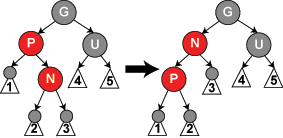
\includegraphics[width=0.5\textwidth]{Red-black_tree_insert_case_4}
	\caption{Transformation of a red-black subtree in case 4 of the insert fixup.}
    \label{insFix4}
  \end{wrapfigure}	
  \paragraph{Case 4}
  The parent \textbf{P} is red but the uncle \textbf{U} is black; also, the new node \textbf{N} is the right child of \textbf{P}, and \textbf{P} is the left child of its parent \textbf{G}. In this case, a left rotation is performed on \textbf{P}. Because Property 4 (Both children of every red node are black) is still violated, \inlinecode{rb-insFixup} is called again on the same subtree. As can be easily seen from the Figures \ref{insFix4} and \ref{insFix5}, Case 4 always leeds on Case 5. The rotation causes some paths (those in the sub-tree labelled ``1'') to pass through the new node where they did not before, but both these nodes are red, so Property 5 (All paths from any given node to its leaf nodes contain the same number of black nodes) is not violated by the rotation.
\end{figure}

\begin{code}
\% CASE \#4\\
rb-insFixup( t( b, Kz, t( r, Ky, Lsy, t( r, Kx, Lsx, Rsx ) ), Uncle ), Tfixed ) :-
\hspace{2ex}rb-insFixup( t( b, Kz, t( r, Kx, t( r, Ky, Lsy, Lsx ), Rsx ), Uncle ), Tfixed ).\\
rb-insFixup( t( b, Kz, Uncle, t( r, Ky, t( r, Kx, Lsx, Rsx ), Rsy ) ), Tfixed ) :-
\hspace{2ex}rb-insFixup( t( b, Kz, Uncle, t( r, Kx, Lsx, t( r, Ky, Rsx, Rsy ) ) ), Tfixed ).
\end{code}

\begin{figure}[h]
  \begin{wrapfigure}{r}{0.5\textwidth}
    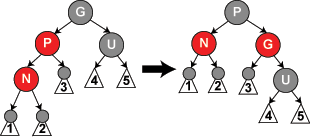
\includegraphics[width=0.5\textwidth]{Red-black_tree_insert_case_5}
    \caption{Transformation of a red-black subtree in case 5 of the insert fixup.}
    \label{insFix5}
  \end{wrapfigure}
  \paragraph{Case 5}
The parent \textbf{P} is red but the uncle \textbf{U} is black, the new node \textbf{N} is the left child of \textbf{P}, and \textbf{P} is also the left child of its parent \textbf{G}. In this case a right rotation is performed on \textbf{G}. Then, the colors of \textbf{P} and \textbf{G} are switched, and the resulting tree satisfies Property 4 (Both children of every red node are black). Property 5 (All paths from any given node to its leaf nodes contain the same number of black nodes) also remains satisfied, since all paths that went through any of these three nodes went through \textbf{G} before, and now they all go through \textbf{P}. In each case, this is the only black node of the three.
\end{figure}

\begin{code}
\% CASE \#5\\
rb-insFixup( t( b, Kz, t( r, Ky, t( r, Kx, Lsx, Rsx ), Rsy ), Uncle ), t( b, Ky, t( r, Kx, Lsx, Rsx ), t( r, Kz, Rsy, Uncle ) ) ).\\
rb-insFixup( t( b, Kz, Uncle, t( r, Ky, Lsy, t( r, Kx, Lsx, Rsx ) ) ), t( b, Ky, t( r, Kz, Uncle, Lsy ), t( r, Kx, Lsx, Rsx ) ) ).
\end{code}

\paragraph{}
If none of the cases 3, 4 or 5 unifies with the subtree given to the \inlinecode{rb-insFixup} predicate, the tree is presumed to satisfy the properties of a red-black tree (except for Property 2 (The root is always black), which is handled separately by the \inlinecode{rb-reblackRoot} predicate on the very end of the insertion ). In this case the tree passes through the `default' predicate, that does not alter it's structure.

\begin{code}
rb-insFixup( T, T ).
\end{code}

\subsubsection[\inlinecode{rb-build}]{Building a red-black tree from a list of elements}
To build a red-black tree from a list of elements, \inlinecode{rb-insert} is called on every element from the list.

\begin{code}
\% rb-build( +List, -Tree )\\
rb-build( L, T ) :-
\hspace{2ex}rb-empty( T0 ),
\hspace{2ex}rb-b( L, T0, T ).\\
rb-b( [], T, T ).\\
rb-b( [ K ], T1, T2 ) :-
\hspace{2ex}rb-insert( T1, K, T2 ).\\
rb-b( [ H \textbar T ], T1, T3 ) :-
\hspace{2ex}rb-insert( T1, H, T2 ),
\hspace{2ex}rb-b( T, T2, T3 ).
\end{code}

\newpage
\subsection{Delete}
\begin{wrapfigure}{r}{0.5\textwidth}
  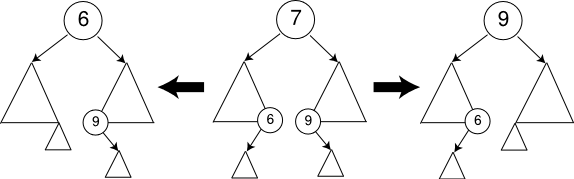
\includegraphics[width=0.5\textwidth]{Binary_search_tree_delete}
  \caption{Binary search tree delete.}
  \label{bstDel}
\end{wrapfigure}
In a normal binary search tree, when deleting a node with two non-leaf children, we find either the maximum element in its left subtree or the minimum element in its right subtree, and move its value into the node being deleted (as shown in Figure \ref{bstDel}). We then delete the node we copied the value from, which must have less than two non-leaf children. Because merely copying a value does not violate any red-black properties, this reduces the problem of deleting to the problem of deleting a node with at most one non-leaf child. It does not matter whether this node is the node we originally wanted to delete or the node we copied the value from.

\subsubsection{rb-delete}
When deleting from a red-black tree several cases may occur most of which are trivial to implement.
\begin{itemize}
\item[:)]
For the remainder of this discussion we can assume we are deleting a node with at most one non-leaf child, which we will call its child (if it has only leaf children, let one of them be its child).
\item[:)]
If we are deleting a red node, we can simply replace it with its child, which must be black. All paths through the deleted node will simply pass through one less red node, and both the deleted node's parent and child must be black, so properties 3 (All leaves, including nulls, are black) and 4 (Both children of every red node are black) still hold.
\item[:)]
Another simple case is when the deleted node is black and its child is red. Simply removing a black node could break Properties 4 (Both children of every red node are black) and 5 (All paths from any given node to its leaf nodes contain the same number of black nodes), but if we repaint its child black, both of these properties are preserved.
\item[:(]
The complex case is when both the node to be deleted and its child are black. We begin by replacing the node to be deleted with its child. We will call (or label) this child (in its new position) \textbf{N}, and its sibling (its new parent's other child) \textbf{S}. In the diagrams below, we will also use \textbf{P} for \textbf{N}'s new parent, \Sl for \textbf{S}'s left child, and \Sr for \textbf{S}'s right child (it can be shown that S cannot be a leaf).
\end{itemize}

The implementation of the delete consists of calling an accessory predicate \inlinecode{rb\-del} and then reblacking the root (by the same predicate as in \inlinecode{rb\_insert}).

\begin{code}
\% rb\_delete( +Tree, +Key, -Tree ).
rb\_delete( T, K, Trb ) :-
\hspace{2ex}rb\_del( T, K, Td ), 
\hspace{2ex}rb\_reblackRoot( Td, Trb ).
\end{code}

There are several simple cases of delete. These do not violate the restrictions of red-black trees.

\begin{code}
\% The Key has not been found
rb\_del( t( b, nil, nil, nil ),  \_, t( b, nil, nil, nil ) ).\\
\% deleting a red node with no children
rb\_del( t( r, K, t( b, nil, nil, nil ), t( b, nil, nil, nil ) ), K, t( b, nil, nil, nil ) ).\\
\% deleting a red node with a left child
rb\_del( t( r, K, Ls, t( b, nil, nil, nil ) ), K, Ls ).\\
\% deleting a red node with a right child
rb\_del( t( r, K, t( b, nil, nil, nil ), Rs ), K, Rs ).\\
\% deleting a black node with a red left child
rb\_del( t( b, K, t( r, Kl, Lsl, Rsl ), t( b, nil, nil, nil ) ), K, t( b, Kl, Lsl, Rsl ) ).\\
\% deleting a black node with a red right child
rb\_del( t( b, K, t( b, nil, nil, nil ), t( r, Kr, Lsr, Rsr ) ), K, t( b, Kr, Lsr, Rsr ) ).
\end{code}

Note: Since a black node cannot have a black `only-child' (It would always violate Property 5 (Every simple path from a given node to its descendant leaves contains the same number of black nodes.)), this case doesn't have to be implemented.

The only case violating the red-black tree properties is the delete of a black node with no children. If doing so, we have to make up for the lost black node. A nice way to implemet this is recoloring the new node \label{double_black}`double black'. The \inlinecode{rb\_delFixup} will take care of that later.

\begin{code}
\% black node with no children
rb\_del( t( b, K, t( b, nil, nil, nil ), t( b, nil, nil, nil ) ), K, t( bb, nil, nil, nil ) ).
\end{code}

\pagebreak
The process of deleting a node with both children as described above is implemented here, along with branching the delete. In both cases this is the place where \inlinecode{rb\_delFixup} is actually called, since these are the places where the recursion is performed. The result of this is, that whatever violations are not repaired, but passed higher, are taken care of in the next step (previous iteration).

\begin{code}
\% deleting a node with both children\\
rb\_del( t( C, K, Ls, Rs ), K, Tfixed ) :-
\hspace{2ex}rb\_maximum( Ls, Max ), 
\hspace{2ex}rb\_del( Ls, Max, Lsd ),
\hspace{2ex}rb\_delFixup( t( C, Max, Lsd, Rs ), Tfixed ).\\
\% branching the delete\\
rb\_del( t( C, K, Ls, Rs ), Kd, Tfixed ) :-
\hspace{2ex}K \textgreater{} Kd, 
\hspace{2ex}rb\_del( Ls, Kd, Lsd ),
\hspace{2ex}rb\_delFixup( t( C, K, Lsd, Rs ), Tfixed ).\\
rb\_del( t( C, K, Ls, Rs ), Kd, Tfixed ) :-
\hspace{2ex}K \textless{} Kd, 
\hspace{2ex}rb\_del( Rs, Kd, Rsd ),
\hspace{2ex}rb\_delFixup( t( C, K, Ls, Rsd ), Tfixed ).
\end{code}
  
\subsubsection{rb-delFixup}

\textit{Note}: In order that the tree remains well-defined, we need that every null leaf remains a leaf after all transformations (that it will not have any children). If the node we are deleting has a non-leaf (non-null) child \textbf{N}, it is easy to see that the property is satisfied. If, on the other hand, \textbf{N} would be a null leaf, it can be verified from the diagrams (or code) for all the cases that the property is satisfied as well.

If both N and its original parent are black, then deleting this original parent causes paths which proceed through N to have one fewer black node than paths that do not. As this violates Property 5 (All paths from any given node to its leaf nodes contain the same number of black nodes), the tree must be rebalanced. There are several cases to consider:

\pagebreak
\paragraph{Case 1}
\textbf{N} is the new root. In this case, we are done. We removed one black node from every path, and the new root is black, so the properties are preserved. This is actually taken care of by the \inlinecode{reblackRoot} predicate at the very end of the \inlinecode{rb\_delete}.

\begin{figure}[h!]
  \begin{wrapfigure}{r}{0.5\textwidth}
    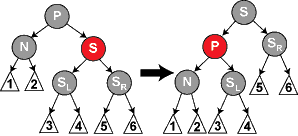
\includegraphics[width=0.5\textwidth]{Red-black_tree_delete_case_2}
    \caption{Transformation of a red-black subtree in case 2 of the delete fixup.}
    \label{delFix2}
  \end{wrapfigure}  
  \paragraph{Case 2}
\textbf{S} is red. In this case we reverse the colors of \textbf{P} and \textbf{S}, and then rotate left at \textbf{P}, turning \textbf{S} into \textbf{N}'s grandparent. Note that \textbf{P} has to be black as it had a red child. Although all paths still have the same number of black nodes, now \textbf{N} has a black sibling and a red parent, so we can proceed to step 4, 5, or 6. (Its new sibling is black because it was once the child of the red S.) In later cases, we will relabel \textbf{N}'s new sibling as \textbf{S}.
\end{figure}

\begin{code}
\% CASE \#2\\
rb\_delFixup( t( b, Kp, N, t( r, Ks, Lss, Rss ) ), t( b, Ks, Tfixed, Rss ) ) :-
\hspace{2ex}N = t( bb, \_, \_, \_ ),
\hspace{2ex}rb\_delFixup( t( r, Kp, N, Lss ), Tfixed ).\\
rb\_delFixup( t( b, Kp, t( r, Ks, Lss, Rss ), N ), t( b, Ks, Lss, Tfixed ) ) :-
\hspace{2ex}N = t( bb, \_, \_, \_ ),
\hspace{2ex}rb\_delFixup( t( r, Kp, Rss, N ), Tfixed ).\\
\end{code}

\pagebreak

\begin{figure}[h]
  \begin{wrapfigure}{r}{0.5\textwidth}
    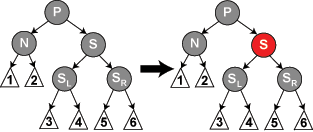
\includegraphics[width=0.5\textwidth]{Red-black_tree_delete_case_3}
    \caption{Transformation of a red-black subtree in case 3 of the delete fixup.}
    \label{delFix3}
  \end{wrapfigure}
  \paragraph{Case 3}
\textbf{P}, \textbf{S}, and \textbf{S}'s children are black. In this case, we simply repaint \textbf{S} red. The result is that all paths passing through \textbf{S}, which are precisely those paths not passing through \textbf{N}, have one less black node. Because deleting \textbf{N}'s original parent made all paths passing through \textbf{N} have one less black node, this evens things up. However, all paths through \textbf{P} now have one fewer black node than paths that do not pass through \textbf{P}, so Property 5 (All paths from any given node to its leaf nodes contain the same number of black nodes) is still violated. To correct this, we perform the rebalancing procedure on \textbf{P}, starting at case 1.
\end{figure}

\begin{code}
\% CASE \#3\\
rb\_delFixup( t( b, Kp, t( bb, Kn, Lsn, Rsn ), t( b, Ks, Lss, Rss ) ),
\hspace{13ex}t( bb, Kp, t( b, Kn, Lsn, Rsn ), t( r, Ks, Lss, Rss ) ) ) :-
\hspace{2ex}Lss = t( b, \_, \_, \_ ),
\hspace{2ex}Rss = t( b, \_, \_, \_ ).\\
rb\_delFixup( t( b, Kp, t( b, Ks, Lss, Rss ), t( bb, Kn, Lsn, Rsn ) ), 
\hspace{13ex}t( bb, Kp, t( r, Ks, Lss, Rss ), t( b, Kn, Lsn, Rsn ) ) ) :-
\hspace{2ex}Lss = t( b, \_, \_, \_ ),
\hspace{2ex}Rss = t( b, \_, \_, \_ ).
\end{code}

\begin{figure}[h]
  \begin{wrapfigure}{r}{0.5\textwidth}
    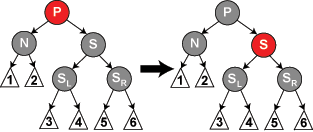
\includegraphics[width=0.5\textwidth]{Red-black_tree_delete_case_4}
    \caption{Transformation of a red-black subtree in case 4 of the delete fixup.}
    \label{delFix4}
  \end{wrapfigure}
  \paragraph{Case 4}
\textbf{S} and \textbf{S}'s children are black, but \textbf{P} is red. In this case, we simply exchange the colors of \textbf{S} and \textbf{P}. This does not affect the number of black nodes on paths going through \textbf{S}, but it does add one to the number of black nodes on paths going through \textbf{N}, making up for the deleted black node on those paths.
\end{figure}

\begin{code}
\% CASE \#4\\
rb\_delFixup( t( r, Kp, N, t( b, Ks, Lss, Rss ) ),
\hspace{13ex}t( b, Kp, N2, t( r, Ks, Lss, Rss ) ) ) :-
\hspace{2ex}N = t( bb, Kn, Lsn, Rsn ), 
\hspace{2ex}N2 = t( b, Kn, Lsn, Rsn ),
\hspace{2ex}Lss = t( b, \_, \_, \_ ),
\hspace{2ex}Rss = t( b, \_, \_, \_ ).\\
rb\_delFixup( t( r, Kp, t( b, Ks, Lss, Rss ), N ), 
\hspace{13ex}t( b, Kp, t( r, Ks, Lss, Rss ), N2 ) ) :-
\hspace{2ex}N = t( bb, Kn, Lsn, Rsn ), 
\hspace{2ex}N2 = t( b, Kn, Lsn, Rsn ),
\hspace{2ex}Lss = t( b, \_, \_, \_ ),
\hspace{2ex}Rss = t( b, \_, \_, \_ ).
\end{code}

\begin{figure}[h]
  \begin{wrapfigure}{r}{0.5\textwidth}
    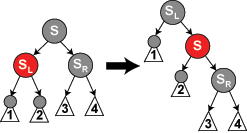
\includegraphics[width=0.5\textwidth]{Red-black_tree_delete_case_5}
    \caption{Transformation of a red-black subtree in case 5 of the delete fixup.}
    \label{delFix5}
  \end{wrapfigure}
  \paragraph{Case 5}
\textbf{S} is black, \textbf{S}'s left child is red, \textbf{S}'s right child is black, and \textbf{N} is the left child of its parent. In this case we rotate right at \textbf{S}, so that \textbf{S}'s left child becomes \textbf{S}'s parent and \textbf{N}'s new sibling. We then exchange the colors of \textbf{S} and its new parent. All paths still have the same number of black nodes, but now \textbf{N} has a black sibling whose right child is red, so we fall into case 6. Neither \textbf{N} nor its parent are affected by this transformation. (Again, for case 6, we relabel \textbf{N}'s new sibling as \textbf{S}.)
\end{figure}

\begin{code}
\% CASE \#5\\
rb\_delFixup( t( Cp, Kp, N, S ), Tfixed ) :-
\hspace{2ex}N = t( bb, \_, \_, \_ ),
\hspace{2ex}S = t( b, Ks, Lss, Rss ),
\hspace{2ex}Lss = t( r, Ksl, Lsl, Rsl ),
\hspace{2ex}Rss = t( b, \_, \_, \_ ),
\hspace{2ex}rb\_delFixup( t( Cp, Kp, N, t( b, Ksl, Lsl, t( r, Ks, Rsl, Rss ) ) ), Tfixed ).\\
rb\_delFixup( t( Cp, Kp, S, N ), Tfixed ) :-
\hspace{2ex}N = t( bb, \_, \_, \_ ),
\hspace{2ex}S = t( b, Ks, Lss, Rss ),
\hspace{2ex}Lss = t( b, \_, \_, \_ ),
\hspace{2ex}Rss = t( r, Ksr, Lsr, Rsr ),
\hspace{2ex}rb\_delFixup( t( Cp, Kp, t( b, Ksr, t( r, Ks, Lss, Lsr ), Rsr ), N ), Tfixed ).
\end{code}

\begin{figure}[h]
  \begin{wrapfigure}{r}{0.5\textwidth}
    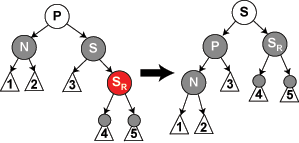
\includegraphics[width=0.5\textwidth]{Red-black_tree_delete_case_6}
    \caption{Transformation of a red-black subtree in case 6 of the delete fixup.}
    \label{delFix6}
  \end{wrapfigure}
  \paragraph{Case 6}
\textbf{S} is black, \textbf{S}'s right child is red, and \textbf{N} is the left child of its parent \textbf{P}. In this case we rotate left at \textbf{P}, so that \textbf{S} becomes the parent of \textbf{P} and \textbf{S}'s right child. We then exchange the colors of \textbf{P} and \textbf{S}, and make \textbf{S}'s right child black. The subtree still has the same color at its root, so Properties 4 (Both children of every red node are black) and 5 (All paths from any given node to its leaf nodes contain the same number of black nodes) are not violated. However, \textbf{N} now has one additional black ancestor: either \textbf{P} has become black, or it was black and \textbf{S} was added as a black grandparent. Thus, the paths passing through \textbf{N} pass through one additional black node.
\end{figure}

\begin{code}
\% CASE \#6\\
rb\_delFixup( t( Cp, Kp, N, S ), 
\hspace{13ex}t( Cp, Ks, t( b, Kp, N2, Lss ), Rss2 ) ) :-
\hspace{2ex}N = t( bb, Kn, Lsn, Rsn ), 
\hspace{2ex}N2 = t( b, Kn, Lsn, Rsn ),
\hspace{2ex}S = t( b, Ks, Lss, Rss ), 
\hspace{2ex}Rss = t( r, Kr, Lsr, Rsr ),
\hspace{2ex}Rss2 = t( b, Kr, Lsr, Rsr ).\\  
rb\_delFixup( t( Cp, Kp, S, N ), 
\hspace{13ex}t( Cp, Ks, Lss2, t( b, Kp, Rss, N2 ) ) ) :-
\hspace{2ex}N = t( bb, Kn, Lsn, Rsn ), 
\hspace{2ex}N2 = t( b, Kn, Lsn, Rsn ),
\hspace{2ex}S = t( b, Ks, Lss, Rss ), 
\hspace{2ex}Lss = t( r, Kl, Lsl, Rsl ),
\hspace{2ex}Lss2 = t( b, Kl, Lsl, Rsl ).
\end{code}

Meanwhile, if a path does not go through \textbf{N}, then there are two possibilities:
\begin{itemize}
\item
It goes through \textbf{N}'s new sibling. Then, it must go through \textbf{S} and \textbf{P}, both formerly and currently, as they have only exchanged colors and places. Thus the path contains the same number of black nodes.
\item
It goes through \textbf{N}'s new uncle, \textbf{S}'s right child. Then, it formerly went through \textbf{S}, \textbf{S}'s parent, and \textbf{S}'s right child (which was red), but now only goes through \textbf{S}, which has assumed the color of its former parent, and \textbf{S}'s right child, which has changed from red to black (assuming \textbf{S}'s color: black). The net effect is that this path goes through the same number of black nodes.
\end{itemize}

Either way, the number of black nodes on these paths does not change. Thus, we have restored Properties 4 (Both children of every red node are black) and 5 (All paths from any given node to its leaf nodes contain the same number of black nodes). The white node in the diagram can be either red or black, but must refer to the same color both before and after the transformation.

\section{Summary}
The work on this implemetation went fairly well. It was not an easy task, particularly \inlinecode{rb\_delete} gave me a hard time, since I had to implement it twice. The first version did not work in some cases and was impossible to debug, because of my horrible coding style. I tried to write the second version a bit more comprehensible and I am pleased with the result. The \inlinecode{rb\_insert} is written ugly but correctly. If anyone would intend to alter it I would recomend rewriting it into a more comprehensible form first. I only implemeted basic operation like insert and delete, because using these it is fairly simple to write more complex ones like merge e.i.

Materials issued in \cite{cepek} gave me a nice inside into red-black trees.

Mostly when writing the documentation I have used materials from \cite{wiki}. (All the pictures and some text are directly copied from there) 


\begin{thebibliography}{9}

  \bibitem{ita}
    Cormen, Leiserson, Rivest, and Stein, 
    \emph{Introduction to Algorithms}
	MIT Press
	
  \bibitem{wiki}
    \url{http://en.wikipedia.org/wiki/Red-black_trees}

  \bibitem{cepek}
    \url{http://kti.mff.cuni.cz/~cepek/ADS1.ppt}

  \bibitem{java}
    \url{http://reptar.uta.edu/NOTES5311/REDBLACK/RedBlack.html}
	
\end{thebibliography}



\end{document}